\section{Data processing and basic results}
\label{section:results}

\begin{table*}[h!]
  \caption{Distribution of non IPv4 frames}
  \label{tab:non:ipv4:frames}
  \centering
  \begin{tabular}{lcc}
    \hline
    {\bf Protocol}                                   & {\bf Number of frames } & {\bf Fraction (\%)} \\
    \hline
    ARP                                              & 136857                  & 48.8 \\
    Cisco Shared Spanning Tree Protocol              & 119385                  & 42.5 \\    
    IPv6                                             & 17034                   & 6.1  \\
    Spanning Tree Protocol (IEEE 802.1D)             & 4774                    & 1.7  \\
    IPX                                              & 1164                    & 0.4  \\
    Cisco Loop                                       & 957                     & 0.3  \\
    Cisco CDP/VTP                                    & 510                     & 0.2  \\
  \end{tabular}
\end{table*}



To perform the preprocessing we have extracted the binary data
and stored it in {\em pdml} (Packet Description Markup Language) 
format - a special XML format which is used to describe the 
contents of the binary representation of frames and packets.

Our next step was to extract needed fields from the XML 
file and store the extracted data in the format which was 
simpler for further analysis. Thus, we have chosen 
JSON (JavaScript Object Notation) format. From PDML
we have extracted the following fields:

\bi
  \im Ethernet source and destination MAC addresses and type field
  \im VLAN identifier and type field
  \im From IP header we have extracted source and destination 
      addresses, version number, length, protocol type, and TTL.
  \im Basic information from GRE and PPP headers (since 
      clients accessing the Internet were using these protocols)
  \im From TCP header we have selected source and destination ports, 
      stream identifier, length, sequence and acknowledgment numbers, 
      as well as flags and window size.
  \im From UDP header source and destination ports, as well as datagram 
      length information were extracted.
\ei

Our next step in preprocessing the data was to extract non IPv4 frames - 
frames for which neither Ethernet type nor VLAN type field were equal to 
{\bf 0x00008000} (this dataset includes packets from all VLANs as well as
packets from native VLAN). Once the data was extracted we binned the 
frames according to protocol types. In Table~\ref{tab:non:ipv4:frames} 
we present the summary results for this data.


\begin{table*}[h!]
  \caption{Distribution of protocols in native VLAN}
  \label{tab:native:vlan}
  \centering
  \begin{tabular}{lcc}
    \hline
    {\bf Protocol}                                   & {\bf Number of frames } & {\bf Fraction (\%)} \\
    \hline
    Cisco Shared Spanning Tree Protocol              & 4774                    & 40.5 \\
    Spanning Tree Protocol (IEEE 802.1D)             & 4774                    & 40.5 \\
    Cisco Loop protocol                              & 957                     & 8.1  \\
    IP (ICMP only)                                   & 640                     & 5.4  \\
    Cisco CDP/VTP                                    & 510                     & 4.3  \\
    ARP                                              & 128                     & 1.1  \\
  \end{tabular}
\end{table*}

\begin{table*}[h!]
  \caption{Frames with invalid MAC addresses}
  \label{tab:invalid:mac}
  \centering
  \begin{tabular}{ccccc}
    \hline
    {\bf Source MAC}       & {\bf Destination MAC }        & {\bf Source IP}        & {\bf Destination IP} &  {\bf Manufacturer}     \\ 
    \hline
30:f9:ed:41:a6:01 & 00:c0:ee:9a:5a:85 & 192.168.5.10 & 192.168.5.151 & Sony/KYOCERA \\
00:30:05:c2:b7:ff & 00:17:c8:03:a0:7b & 192.168.18.7 & 192.168.18.34 & Fujitsu/KYOCERA \\
00:15:58:67:5f:14 & 00:c0:ee:9a:5a:85 & 192.168.5.3 & 192.168.5.151 & FOXCONN/KYOCERA \\
    \hline
  \end{tabular}
\end{table*}



The next step in preprocessing of the data was to exclude the frames 
for the native VLAN from the traces. Thus, we have filtered out 
the frames for which Ethernet type was not equal to {\bf 0x00008100}.
It turned out that the fraction of frames without VLAN tag was rather 
small and constituted only $0.06 \%$ of the total number of frames in 
the trace. Since native VLAN was used only for management purposes
we excluded it from further analysis. However, in Table~\ref{tab:native:vlan} we show 
the  distribution of packet types seen in the native VLAN.

\begin{table*}[h!]
  \caption{Distribution of top applications used in the network}
  \label{tab:apps}
  \centering
  \begin{tabular}{cccccc}
    \hline
    {\bf TCP port} & {\bf Frequency } & {\bf Application} & {\bf UDP port} & {\bf Frequency} & {\bf Application}       \\
    \hline
         13000     & 11599            &  Kaspersky        &        53      &      27960      & DNS                     \\
         443       & 10128            &  HTTPS            &        137     &      6589       & NetBIOS                 \\
          88       & 9700             &  Kerboros         &       389      &      1350       & LDAP                    \\
          80       & 6938             &  HTTP             &     15000      &      804        & Kaspersky Network Agent \\
          445      & 5581             &  Microsoft SMB    &        88      &      166        & Kerboros                \\
          135      & 940              &  MS RPC           &       123      &      146        & NTP                     \\
          389      & 880              &  LDAP             &      13000     &      50         & Kaspersky               \\
          49155    & 694              &  Microsoft-DC     &      138       &      21         & NetBIOS                 \\
          139      & 682              &  Netbios          &      443       &      16         & QUIC                    \\
    \hline
  \end{tabular}
\end{table*}

Instead, next we turned our attention to frames with invalid MAC addresses. 
By invalid MAC address we mean those MAC addresses which are not multicast or 
broadcast addresses received at the trunk interface of the router with 
destination unicast MAC addresses not of router's own MAC addresses. 
Upon filtering the data we have found that there were two such 
destination unicast MAC addresses. We hypothesize that such frames could have been
received at the trunking interface due to the following reasons. The MAC
address table of the switches (i) did not contain a record for the destination 
MAC address and so it was flooded to all ports except the port from which 
the frame was received; (ii) wrong mapping for the destination MAC 
address and outgoing interfaces could have existed and so it was 
forwarded into the wrong port of the switch and thus was received at the 
trunk port of the router. The two invalid MAC addresses we have discovered are: 
{\bf 00:17:c8:03:a0:7b} and {\bf 00:c0:ee:9a:5a:85}. We leave this 
investigation to the network administrators.


Our next step of data preprocessing was to find for every packet being 
forwarded a corresponding pair: Note, our trace contained two copies 
of a packet for which the source and destination IP addresses where within 
the {\em 192.168.0.0/16} subnetwork with a difference that TTL was reduced 
by one for one of the packets, and the Ethernet header was recalculated. 
Thus, by filtering out the duplicates we were able to excluded the 
possibility of overcounting the number of bytes carried in TCP and 
UDP streams, and other transport protocols. To perform this filtering step, 
we merely found all packets whose source and destination addresses where within 
the subnetwork {\em 192.168.0.0/16} and filtered out frames for which 
source MAC address was not equal to the MAC address of the VLAN server
(note, all VLAN interfaces were assigned the same MAC address). 
Thus, effectively leaving only one copy of the packet being forwarded 
between the subnetworks in the trace. Our resulting trace was reduced by
$35.4 \%$, and now contained $12190001$ frames.

Once again we have searched for frames with invalid MAC
addresses (we have introduced the term invalid MAC addresses in the
previous paragraphs). In Table~\ref{tab:invalid:mac} we list these
MAC addresses as well as corresponding IP addresses found in such
frames, and manufacture's name. Obviously, such disripancy is strange.

\begin{figure}[!hbt]\centering
  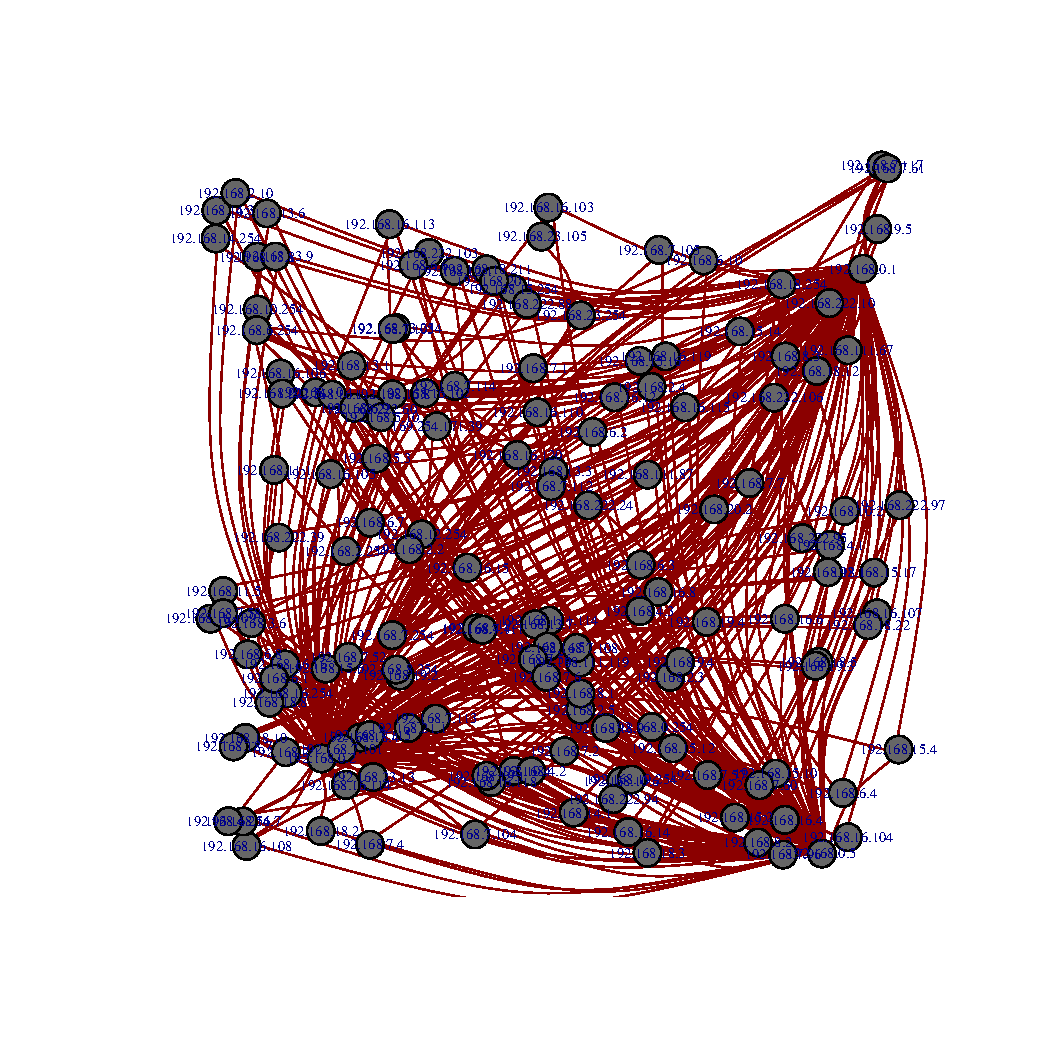
\includegraphics[width=0.45\textwidth]{graphics/interaction_between_local_computers_over_tcp.pdf}
  \caption{Interaction between computers in different VLANs over TCP}
  \label{fig:interaction}
\end{figure}

\eat{
\begin{figure}[!hbt]\centering
  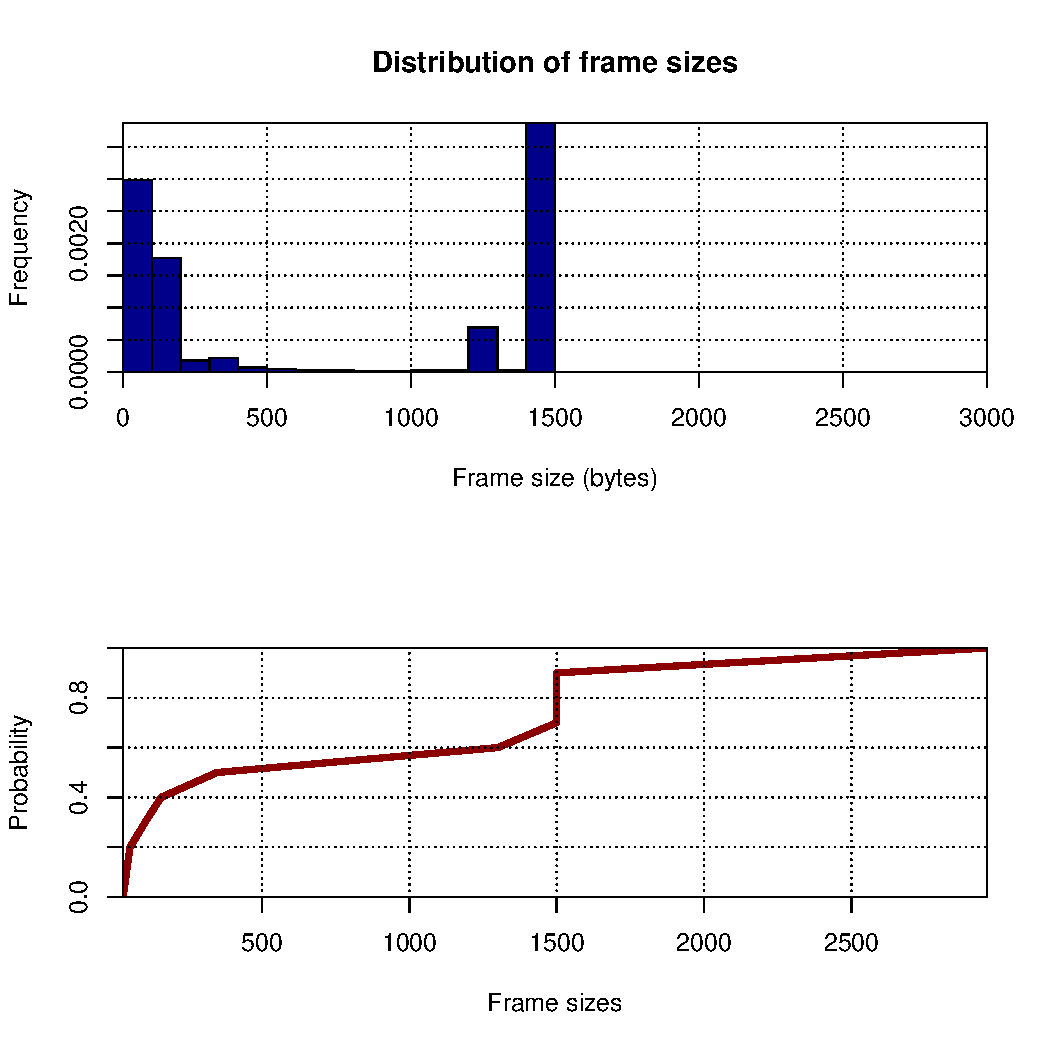
\includegraphics[width=0.45\textwidth]{graphics/distribution_of_frame_sizes.pdf}
  \caption{Distribution of frame sizes}
  \label{fig:frame_sizes}
\end{figure}
}

For the cleaned data, our first step was to take a look at the distribution of TCP and UDP applications and the number of bytes these 
applications transmitted. Thus, in Table~\ref{tab:apps} we show the distribution of $9$ most used UDP and TCP applications. We examened 
both inter-VLAN and Internet traffic. We observed that while most of hosts were not actively connected to the Internet, using the VPN 
connections, $15366$ connection attemps were made towards the Internet (only TCP SYN packet was captured, which was dropped by the 
firewall). This could be an indication that quite a lot of connections are made in fact in a stealth mode on users' computers. Next, we 
have computed the adjacency graph for computers which were interacting over TCP in the local network (an interaction here means that at 
least one TCP/UDP connection between the pair of computers existed). \eat{In Figure~\ref{fig:interaction} we demonstrated the graph of 
interaction for TCP connections only.} As it was expected, only few computers (servers) were accepting all TCP connection, with a small 
fraction of computers were interacting between each other. Upon expecting closely the logs we have found few interesting things: (i) at 
least one machine had misconfigured address (it was using self generated IP addresses with the prefix $169.254.171.0/24$); (ii) 
only two machines were interacting with non-server computers $192.168.23.13$ and $192.168.3.6$ using ports $139$ and $445$.

\begin{figure}[!hbt]
  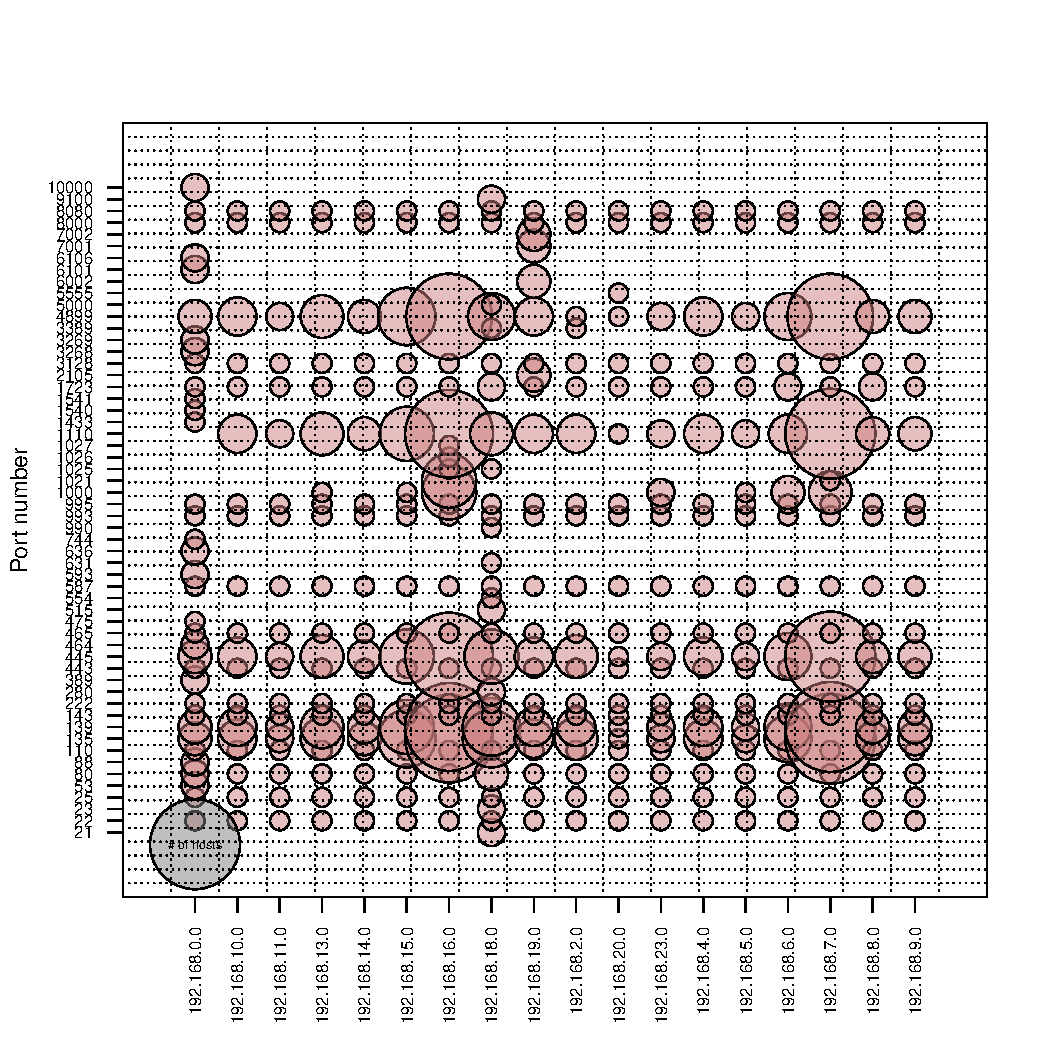
\includegraphics[width=0.45\textwidth]{graphics/bubble_plot_distribution_of_open_ports.pdf }
  \caption{Distribution of ports used in the network}
  \label{fig:ports}
\end{figure}   

Next we computed the distribution of the packet sizes for packets with valid IP addresses. Interestingly there were frames which were larger than maximum allowed Ethernet frames 
size (so called jumbo frames). Around $10\%$ of the IPv4 packet were larger than $1500$ bytes. Finally, we have build the distribution 
of destination ports used in the packets. In Figure~\ref{fig:ports} we show this distribution.


